\documentclass[12pt]{article}
\usepackage[margin=1in]{geometry}
\usepackage{setspace}
\onehalfspacing

% Start of preamble
%==========================================================================================%
% Required to support mathematical unicode
\usepackage[warnunknown, fasterrors, mathletters]{ucs}
\usepackage[utf8x]{inputenc}

\usepackage[dvipsnames,table,xcdraw]{xcolor}

% Standard mathematical typesetting packages
\usepackage{amsmath,amssymb,amscd,amsthm,amsxtra, pxfonts}
\usepackage{mathtools,mathrsfs,dsfont,xparse}

% Symbol and utility packages
\usepackage{cancel, textcomp}
\usepackage[mathscr]{euscript}
\usepackage[nointegrals]{wasysym}
\usepackage{apacite}

% Extras
\usepackage{physics}  
\usepackage{tikz-cd} 
\usepackage{microtype}
\usepackage{enumitem}
\usepackage{titling}
\usepackage{graphicx}

% Fancy theorems due to @intuitively on discord
\usepackage{mdframed}
\newmdtheoremenv[
backgroundcolor=NavyBlue!30,
linewidth=2pt,
linecolor=NavyBlue,
topline=false,
bottomline=false,
rightline=false,
innertopmargin=10pt,
innerbottommargin=10pt,
innerrightmargin=10pt,
innerleftmargin=10pt,
skipabove=\baselineskip,
skipbelow=\baselineskip
]{mytheorem}{Theorem}

\newenvironment{theorem}{\begin{mytheorem}}{\end{mytheorem}}

\newtheorem{corollary}{Corollary}
\newtheorem{lemma}{Lemma}

\newtheoremstyle{definitionstyle}
{\topsep}%
{\topsep}%
{}%
{}%
{\bfseries}%
{.}%
{.5em}%
{}%
\theoremstyle{definitionstyle}
\newmdtheoremenv[
backgroundcolor=Violet!30,
linewidth=2pt,
linecolor=Violet,
topline=false,
bottomline=false,
rightline=false,
innertopmargin=10pt,
innerbottommargin=10pt,
innerrightmargin=10pt,
innerleftmargin=10pt,
skipabove=\baselineskip,
skipbelow=\baselineskip,
]{mydef}{Definition}
\newenvironment{definition}{\begin{mydef}}{\end{mydef}}

\newtheorem*{remark}{Remark}

\newtheorem*{example}{Example}

% Common shortcuts
\def\mbb#1{\mathbb{#1}}
\def\mfk#1{\mathfrak{#1}}

\def\bN{\mbb{N}}
\def \C{\mbb{C}}
\def \R{\mbb{R}}
\def\bQ{\mbb{Q}}
\def\bZ{\mbb{Z}}
\def \cph{\varphi}
\renewcommand{\th}{\theta}
\def \ve{\varepsilon}
\newcommand{\mg}[1]{\| #1 \|}

% Often helpful macros
\newcommand{\floor}[1]{\left\lfloor#1\right\rfloor}
\newcommand{\ceil}[1]{\left\lceil#1\right\rceil}
\renewcommand{\qed}{\hfill\qedsymbol}
\renewcommand{\P}{\mathbb P\qty}
\newcommand{\E}{\mathbb{E}\qty}
\newcommand{\Cov}{\mathrm{Cov}\qty}
\newcommand{\Var}{\mathrm{Var}\qty}

% Sets
\usepackage{braket}

\graphicspath{{/}}
\usepackage{float}

\newcommand{\SET}[1]{\Set{\mskip-\medmuskip #1 \mskip-\medmuskip}}

% End of preamble
%==========================================================================================%

% Start of commands specific to this file
%==========================================================================================%

\usepackage{listings}
\lstset{
    breaklines=true,          % Enable word wrapping
    basicstyle=\ttfamily,     % Use a typewriter font
    columns=fullflexible,     % Adjust spacing for text
    frame=single              % Optional: Add a frame around the text
}

%==========================================================================================%
% End of commands specific to this file

\title{CSE 447 HW3}
\date{\today}
\author{Rohan Mukherjee}

\begin{document}
    \maketitle
    \subsection*{1.2}
    I chose the option to replace the key, query, and value projection matrices with small, fully connected neural networks, with ReLU activations in between. Here is a picture of the architecture:
    \begin{figure}[H]
        \centering
        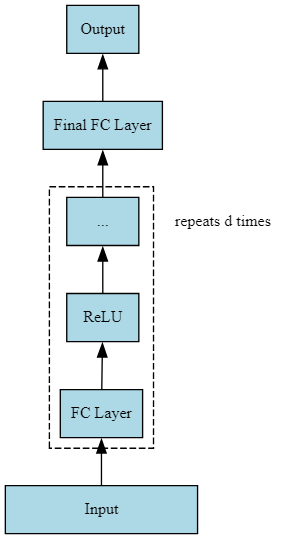
\includegraphics[width=0.4\textwidth]{nn.png}
        \caption{Neural network architecture for key, query, and value}
    \end{figure}

    This is a relatively simple model, but it should add some non-lineararity to the transformer's attention that might end up changing some things. 

    My experiment was to use this architecture with a tuneable parameter $d$, which represents the number of hidden layers, and compute the perplexity of the model on the test and dev set, as well as the last loss on the training set, and plot it against $d$. I chose $d \in \SET{1, 4, 7, 10, 13, 17, 20, 23, 26, 30}$ and here are my results:
    \begin{figure}[H]
        \centering
        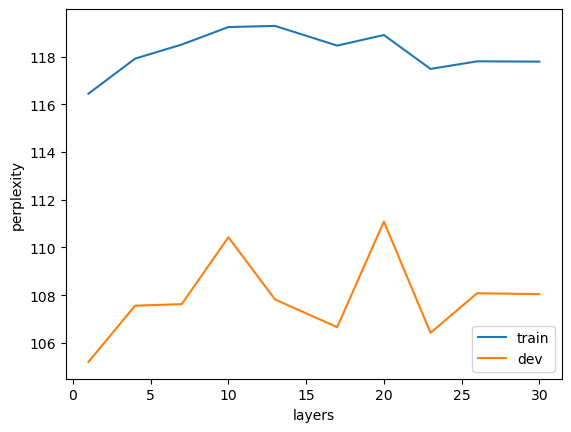
\includegraphics[width=0.5\textwidth]{ppl_vs_layers.png}
        \caption{Perplexity of the model on the test and dev set vs Layers}
    \end{figure}

    \begin{figure}[H]
        \centering
        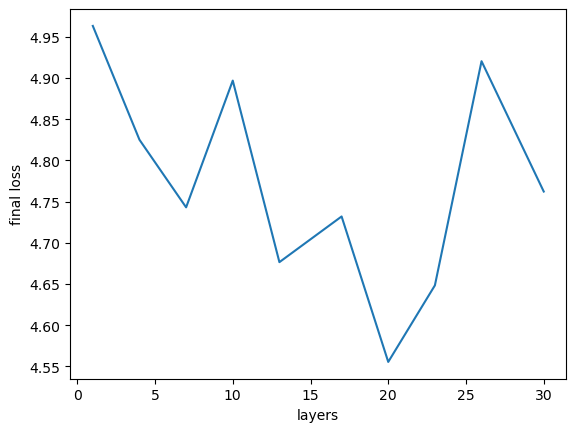
\includegraphics[width=0.5\textwidth]{loss_vs_layers.png}
        \caption{Loss of the model on the training set vs Layers}
    \end{figure}
    As you can see, the training and dev perplexity remain relatively constant, while the last training loss has no clear pattern, increasing up and down spontaneously throughout increasing layers. I think this shows that there is no real need to make the key, query, and value projections more complex, since they are already working fine, and making them more complex doens't seem to help. 

    Here is one generation from each model from $d=1$ to $d=30$:
    \begin{lstlisting}
        layers = 1
        <START> <UNK> from mine , to King It MOWBRAY : if honest very breath to your oath pronounced being sir , I would in the <UNK> Does Which fly , and hear that <UNK> enough ? <STOP>
        <START> O lord ! and Clifford , hours of your hand , from and sir , Whither , as Leontes <UNK> . <STOP>
        <START> farewell : disease 's the save for my loved him ; With poor <UNK> of us and in pay so , for the soften spirit and thy great help . <STOP>
    \end{lstlisting}
    \begin{lstlisting}
        layers = 4
        <START> but he should go . <STOP>
        <START> ROMEO MOWBRAY : Now , themselves ! <STOP>
        <START> : hath not go <UNK> Thou contract that <UNK> queen . <STOP>
    \end{lstlisting}
    \begin{lstlisting}
        layers = 7
        <START> How steal Thus if you <UNK> the <UNK> with as noble Aumerle . <STOP>
        <START> BENVOLIO : I must have you , my Rome to court , Thou Will not let me , Which charge them <UNK> that speak to black own <UNK> . <STOP>
        <START> May name is from him that he is by the remorse in my rather . <STOP>
    \end{lstlisting}
    \begin{lstlisting}
        layers = 10
        <START> CLAUDIO : You told cold ' what , Would she is a houses 'd you done o'er a QUEEN ELIZABETH : Which <UNK> what , and that stands such of blood , loins . <STOP>
        <START> and they lose his followers : our words late <UNK> purpose of for this lie so of we stood my father to myself , Thus He slaughter That more over <UNK> Of great <UNK> 'd , By virtuous And wenches i : Look themselves . <STOP>
        <START> BISHOP OF heartily a loved the gods toward the <UNK> with care to him set your Duke of Tybalt shall wake of my their food . <STOP>
    \end{lstlisting}
    \begin{lstlisting}
        layers = 13
        <START> MENENIUS : Now , 't is honours praise the king , An little better seated she was condemn hast I 'll not at the crown , the house see like made so it not more earth . <STOP>
        <START> Can your art not speak to be o ' ' ' dead more , of rise Brandon , you make good rain : Strike the rabble . <STOP>
        <START> so others with follow me by France . <STOP>
    \end{lstlisting}
    \begin{lstlisting}
        layers = 17
        <START> QUEEN MARGARET : about him me me , ! <STOP>
        <START> <UNK> thee , for my damned centre of the longer say he <UNK> of sweet daughters ; by eye is winter is heaven , fool , though upon prepared for thou friend . <STOP>
        <START> for their Trust weight , on , this Anne ; Hark , young <UNK> of <UNK> to accuse thee to tears ; Within them your brother lives ; bear my contrary . <STOP>
    \end{lstlisting}
    \begin{lstlisting}
        layers = 20
        <START> DUKE VI : The day with my thing to the possession : My Son ; and king ? <STOP>
        <START> MARCIUS : Let me Capulet , over the young Who ? <STOP>
        <START> KING RICHARD ELIZABETH : Edward 's death : dead thank Warwick , I can ? <STOP>
    \end{lstlisting}
    \begin{lstlisting}
        layers = 23
        <START> KING RICHARD III : name ? <STOP>
        <START> WARWICK : Sir than this matter flowers . <STOP>
        <START> Methought Thou puissant morning , and every prison appear , the rest Must that , to grant it was well . <STOP>
    \end{lstlisting}
    \begin{lstlisting}
        layers = 26
        <START> I 'll end the arms , at the not up , in thee authority , -- Third lusty slain ? <STOP>
        <START> Yet speak ? <STOP>
        <START> your honour thine more banished ? <STOP>
    \end{lstlisting}
    \begin{lstlisting}
        layers = 30
        <START> KING EDWARD : <STOP>
        <START> Second Murderer : My field , spoke with dust the coat , If I have most those he must . <STOP>
        <START> Be more <UNK> the victory me offer up to speak . <STOP>
    \end{lstlisting}

    Expectedly, since these models have very simliar perplexities and losses, these generations also look very similar. This cements the fact that there is not really a good reason to use a more complicated version of the $Q, K, V$ than just the dot product, since you don't get any gains but get penalized by a lot higher training time. 


    \subsection*{2.1}
    In greedy decoding, I got:
    \begin{lstlisting}
        ['Ryan was called by his friend to skip work one day.'] ==> ['\n\n"I was like, \'I\'m going to go to work tomorrow,\'" he said.']
        ['Ryan was called by his friend to skip work one day.'] ==> ['\n\n"I was like, \'I\'m going to go to work tomorrow,\'" he said.']
        ['Ryan was called by his friend to skip work one day.'] ==> ['\n\n"I was like, \'I\'m going to go to work tomorrow,\'" he said.']
        ['Ryan was called by his friend to skip work one day.'] ==> ['\n\n"I was like, \'I\'m going to go to work tomorrow,\'" he said.']
    \end{lstlisting}
    As you can see, the generation is the same each time. This is because greedy decoding is deterministic. 

    For vanilla sampling, I got:
    \begin{lstlisting}
        ['Ryan was called by his friend to skip work one day.'] ==> ['\n\n"Let\'s walk through the window," the banner states (it didn\'t say that at']
        ['Ryan was called by his friend to skip work one day.'] ==> [' Tucked inside a basement window, he found a packed pack of cigarettes on a tin counter in the']
        ['Ryan was called by his friend to skip work one day.'] ==> [' He said he wanted to enroll in school next Thursday.\n\nPolice said a woman and her child']
        ['Ryan was called by his friend to skip work one day.'] ==> [' The person had taken him on a hike.\n\nWas filming normal? Yep, except that the']
        ['Ryan was called by his friend to skip work one day.'] ==> [' Employees of Target were telling him that Garrett wanted to take action on the education rights of low-income']
        ['Ryan was called by his friend to skip work one day.'] ==> [' He heard his friend was in trouble and put on a so-called militia, intending to die,']
        ['Ryan was called by his friend to skip work one day.'] ==> [' In a bit of an odd coincidence, he was engaged to workers at Franz Schoffel, who']
        ['Ryan was called by his friend to skip work one day.'] ==> [' The next morning, he wrote a letter to his employer requesting that he lay off 15 hours of work']
        ['Ryan was called by his friend to skip work one day.'] ==> [' His second time around broke him. The last he went out by himself was in 1991, when he']
        ['Ryan was called by his friend to skip work one day.'] ==> [" The two met at McDonald's kitchen. They walked into a small restaurant for lunch there. When a"]
    \end{lstlisting}
    There is a lot of variation in these generations. In the beginning, they make no sense, but near the end a lot of them are very choerent. For example, let's walk through the window isn't a very common thing people would say. But the last one is a logically coherent sentence. Also, there are very few repetitions, and as expected, since there are so many words to sample from, sometimes you get words that aren't even remotely related to the question. Like the example when it starts talking about Garett at target. 

    For temperature sampling, I got:
    \begin{lstlisting}
        ['Ryan was called by his friend to skip work one day.'] ==> ['\n\n"I told him if I listened to the job, (it would pay him) $']
        ['Ryan was called by his friend to skip work one day.'] ==> [' The hunger strike was held in a tunnel deep beneath Northeast Cleveland, which was hosting a public hearing.']
        ['Ryan was called by his friend to skip work one day.'] ==> [' He said he wanted to enroll in school.\n\n"I didn\'t feel safe and didn\'t']
        ['Ryan was called by his friend to skip work one day.'] ==> [' The person had taken him on a hike.\n\nWas filming normal?\n\nAnyone who saw']
        ['Ryan was called by his friend to skip work one day.'] ==> ['\n\n"I said, \'Well, how about you head to the cafeteria?\'" Williams said.']
        ['Ryan was called by his friend to skip work one day.'] ==> [' He heard his friend was in trouble and was on a business trip.\n\nWhen Bremming']
        ['Ryan was called by his friend to skip work one day.'] ==> [' In a conversation with his girlfriend, the former bluesman said that it was "off the cuff"']
        ['Ryan was called by his friend to skip work one day.'] ==> [' The next morning, he wrote a letter to his employer requesting that he stay home, according to Yahoo']
        ['Ryan was called by his friend to skip work one day.'] ==> [' His second time around was on a sports team he was playing against and never was able to get a']
        ['Ryan was called by his friend to skip work one day.'] ==> [" The two met at McDonald's, where he said he was forced to give up work to buy a"]
    \end{lstlisting}
    These make sense more often than the vanilla sampling, but are still fairly nonsensical. Vanilla sampling by definition is just $t = 1$. On the other hand, if WLOG $x_1$ is the maximum coordinate of $x = (x_1, \ldots, x_n)$ the input vector, then:
    \begin{align*}
        \frac{e^{x_i/t}}{\sum_{j=1}^n e^{x_j/t}} = \frac{e^{(x_i-x_1)/t}}{\sum_{j=1}^n e^{(x_j-x_1)/t}}
    \end{align*}
    Assuming that no two entries of $x$ are equal, we can see that $e^{(x_i-x_1)/t} \to 0$ as $t \to 0^+$ as $x_i - x_1 < 0$ for $i \neq 1$, and $1$ for $x = 1$. Thus, with $t \to 0^+$, temperature sampling will put all the weight on the most likely word, which is just greedy sampling. 

    Here are some of the generations for top $k$ sampling, with $k = 20$:
    \begin{lstlisting}
        ['Ryan was called by his friend to skip work one day.'] ==> ['\n\n"I told him if I got to the job, he\'d tell me to skip lunch']
        ['Ryan was called by his friend to skip work one day.'] ==> [" The second time, however, he didn't make it because he'd lost interest in his job."]
        ['Ryan was called by his friend to skip work one day.'] ==> [' He said he wanted to come home as soon as possible to have coffee, a meal and to do']
        ['Ryan was called by his friend to skip work one day.'] ==> [' The police had taken him on a search warrant that had to be approved as part of the search for']
        ['Ryan was called by his friend to skip work one day.'] ==> ['\n\n"I said, \'Well, how about you get a job,\' " he said,']
        ['Ryan was called by his friend to skip work one day.'] ==> [" He didn't. But, at night, on a Saturday morning, he would stay awake at a"]
        ['Ryan was called by his friend to skip work one day.'] ==> [' In a conversation that led to his dismissal, they became good friends. In September 2008, the three']
        ['Ryan was called by his friend to skip work one day.'] ==> [' The next morning, he was arrested and charged with DUI after being charged with driving under the influence.']
        ['Ryan was called by his friend to skip work one day.'] ==> [' His job title was "Chief Financial Officer." He went out into the woods in the spring of 1989']
        ['Ryan was called by his friend to skip work one day.'] ==> [" The two met at McDonald's, but he said he didn't even notice the waitress. When he"]
    \end{lstlisting}
    For top $k$ sampling, $k = 1$ will be greedy decoding, since with only one word to sample from, the mode will always choose that word, and by definition this is the most likely word (its the top 1). On the other hand, purely vanilla sampling would just be sampling from the entire distribution, so that would be $k = $ the length of the vocabulary. 

    Here are some generations, with $p = 0.7$:
    \begin{lstlisting}
        ['Ryan was called by his friend to skip work one day.'] ==> ['\n\n"I told him I had a game plan for my game day and I told him,']
        ['Ryan was called by his friend to skip work one day.'] ==> [' The owner said, "This is the guy who shot us, who didn\'t want to do this']
        ['Ryan was called by his friend to skip work one day.'] ==> [" He said he wanted to skip school one day. He said he didn't want to waste time,"]
        ['Ryan was called by his friend to skip work one day.'] ==> [' The person had taken him to the hospital.\n\nZimmerman said the couple had planned to']
        ['Ryan was called by his friend to skip work one day.'] ==> ['\n\n"I said, \'Well, how about you get a job,\' " Williams said.']
        ['Ryan was called by his friend to skip work one day.'] ==> [" He didn't follow through with his contract because he wasn't going to get the money, but instead"]
        ['Ryan was called by his friend to skip work one day.'] ==> [' In a bit of an odd coincidence, he was having a car accident when, in the back seat']
        ['Ryan was called by his friend to skip work one day.'] ==> [' The next morning, he wrote a letter to his employer demanding that he show up at the end of']
        ['Ryan was called by his friend to skip work one day.'] ==> [" His second time around, he couldn't finish her on time, and she was still too tired to"]
        ['Ryan was called by his friend to skip work one day.'] ==> [" The two met at McDonald's, but he said he didn't even notice the waitress. When he"]
    \end{lstlisting}
    For top-p sampling, if $p=1$, then this is equivalent to vanilla sampling, since $p=1$ just gives the entire distribution. On the other hand, if $p = 0$, then this is equivalent to greedy decoding, since any set of words will have cumulative probability greater than $0$, so the smallest number will be 1, and if we order the words in decreasing order of probability, this will just pick the first word, i.e. the most likely word. This is just greedy decoding.

    To be honest, the nucleus sampling seems to work best. Theoretically, it combines the best part about top $k$ sampling while avoiding the possibliity that $k$ is just way too big, or way too small, not encompassing enough reasonable words. Vanilla sampling can just be too wild, which can be controlled by temperature. So a perfect mix would be nucleus sampling with temperature, but since that wasn't an option, the nucleus sampling seems to work best. The generations mostly seem to respond to the question, and they are very coherent, as you can see above. Greedy on the other hand just repeats the same thing, which isn't very useful, since people don't really talk like that. It would never be able to generate an interesting story. 

    \subsection*{2.2.2.}
    Here is a table of the Rouge scores for the different models. I didn't make this a graph because it really doesn't make sense for this to be a graph. What would go on the $x$-axis? You would think parameters, but the parameters are the same for 3 of the models. So it is here as a table:
    \begin{table}[h!]
        \centering
        \begin{tabular}{|l|c|c|c|c|}
        \hline
        \textbf{Model} & \textbf{ROUGE-1} & \textbf{ROUGE-2} & \textbf{ROUGE-L} & \textbf{ROUGE-L Sum} \\ \hline
        Qwen 1.5b & 0.2664 & 0.0840 & 0.1858 & 0.2162 \\ \hline
        Base GPT2 & 0.1890 & 0.0308 & 0.1220 & 0.1602 \\ \hline
        KD Tuned GPT2 & 0.2315 & 0.0553 & 0.1457 & 0.1840 \\ \hline
        Real Data Tuned GPT2 & 0.2511 & 0.0654 & 0.1587 & 0.2330 \\ \hline
        \end{tabular}
        \caption{ROUGE Scores for Different Models}
        \label{tab:rouge_scores}
    \end{table}
    As expected, the teacher model does the best out of all of them. It is really quite impressive, but also has a gigantic overhead, having $1.5$ parameters, vs the 117 million of GPT2. The base GPT2 does the worst, which is expected, since it has a smaller understanding of language than the Qwen model. However, fine-tuning this base model improves the performance drastically. The most interesting thing I see in this table is that we can achieve nearly equal scores across the board with KD tuned GPT2 and Real data tuned GPT2. Knowledge distillation can be entirely automated once you have a large model that has a good understanding of language, while getting human made summaries would be a large undertaking. This is great news for people who want to train a smaller model. 
\end{document}